

\subsection{ID Provider}
An aspect of working with \gls{dash} that can be slightly annoying is the use of id-strings.
The example below shows how the two id-strings \code{graph-content} and \code{dropdown-selection} are used when defining the components and when creating the callback.
\begin{listing}[H]
    \begin{minted}{python}
        app.layout = html.Div([
            html.H1(children='Title of Dash App', style={'textAlign':'center'}),
            dcc.Dropdown(df.country.unique(), 'Canada', id='dropdown-selection'),
            dcc.Graph(id='graph-content')
        ])

        @callback(
            Output('graph-content', 'figure'),
            Input('dropdown-selection', 'value')
        )
        def update_graph(value):
            dff = df[df.country==value]
            return px.line(dff, x='year', y='pop')
    \end{minted}
    \caption{Code showing the use of id string \cite{plotlyMinimalDashApp}}
\end{listing}

Modern \glspl{ide} like \gls{vscode} are capable of providing autocomplete suggestions, speeding up the code writing.
This works really well in for variable and property names, but not for strings.
For larger \gls{dash} projects name collisions can be a problem, and renaming a component through search and replace is not always straight forward.
To solve this annoyance a helper class called \code{IdProvider} was created.

Whenever a new attribute is accessed, like \code{IdProvider.variable1}, a new id-string is generated and returned as shown in Figure \ref{fig:idproider_a} and \ref{fig:idproider_c}.
When the program is finished, the \code{IdProvider.generate_code()} automatically generates the code for the \code{KnownIds} class, using \gls{jinja} templates with output as shown in Figure \ref{fig:idproider_b}.
The \code{KnownIds} is used for typing and have a property matching each of the attributes accesed through \code{IdProvider}.
As the \code{IdProvider} inherits from \code{KnownIds} this makes it possible to use autocomplete anv variable renaming on future calls to \code{IdProvider.variable1} as shown in \ref{fig:idproider_d}.
The \code{StrWithChilren} class is a subclass of \code{str} that makes it possible to add children to the id-string, such as \code{variable3.variable4} shown in Figure \ref{fig:idproider_b}.

\begin{figure}[H]
    \centering
    \subcaptionbox{Code on first run \label{fig:idproider_a}}{
        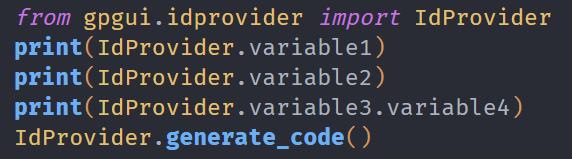
\includegraphics[width=0.45\textwidth]{figures/idp/idp1.png}

    }
    \subcaptionbox{Code on following runs, red color is from linter recognizing names \label{fig:idproider_b}}{
        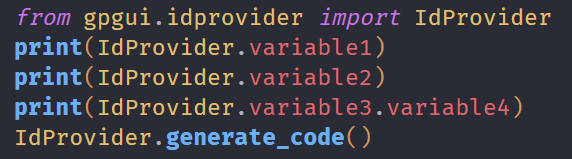
\includegraphics[width=0.45\textwidth]{figures/idp/idp2.png}
    }


    \subcaptionbox{Output from \textbf{(a)} or \textbf{(b) \label{fig:idproider_c}}}{
        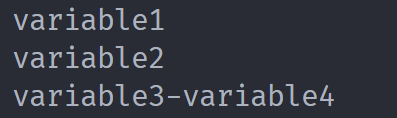
\includegraphics[width=0.4\textwidth]{figures/idp/idp4.png}
    }

    \subcaptionbox{Autogenerated after first run \label{fig:idproider_d}}{
        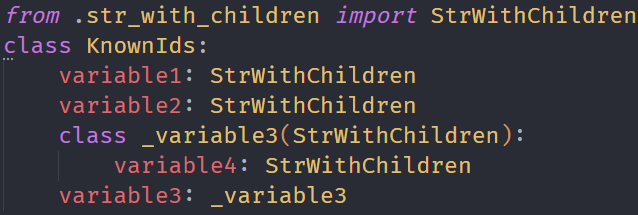
\includegraphics[width=0.45\textwidth]{figures/idp/idp3.png}

    }

    \caption{Visualization of the \code{IdProvider} class}
\end{figure}



